\documentclass[a4paper]{article}
\usepackage{graphicx}
\usepackage{url}
\usepackage{color}

\begin{document}

\title{The Deviation of China Map as a Regression Problem}
\author{Wu Yongzheng}

\maketitle

\section{The Problem}

\section{Notation}
We need to find out two functions, $f_x(x,y)$ and $f_y(x,y)$, to describe the
deviation. $x$ and $y$ are the true longitude and latitude respectively.
$f_x(x,y)$ and $f_y(x,y)$ are the deviation delta at point $(x,y)$.
In other words, if $(x,y)$ is the true coordinate, then
$(x+f_x(x,y),y+f_y(x,y))$ is the deviated coordinate.
Since $|f_x(x+d,y)-f_x(x,y)|$ is much smaller than $d$ (and same for $y$)
we can also
use the two functions to calculate the true coordinate from a deviated
coordinate.
Let $(x,y)$ be the deviated coordinate, $(x-f_x(x,y),y-f_y(x,y))$ is the
true coordinate.

We first solve the functions in one dimension by setting one parameter to be
constant.
I.e. instead of solving $f_x(x,y)$ directly, we first solve $f_x(x,c)$
and $f_x(c,y)$, where $c$ is a constant.
For example, we will look at $f_x(x,39.36)$ and $f_x(110.16,y)$.
Similarly, we will solve $f_y(x,c)$ and $f_y(c,y)$ before $f_y(x,y)$.

In the following analysis, we will use octave.
All the data used in the analysis has already been posted in my previous
article\footnote{url}.

\section{The four 1D cases}
\subsection{$f_x(const,y)$}
$f_x(const,y)$ looks like to be the simplest, so we solve it first.

\noindent
\verb|> data=load("-ascii", "iny-f-110.txt");| \\
\verb|> y=data(:,2);| \\
\verb|> dx=data(:,3);| \\
\verb|> plot(y,dx)| \hfill Figure~\ref{fig:fxy-degree}(left)

\begin{figure}[htb]
\begin{center}
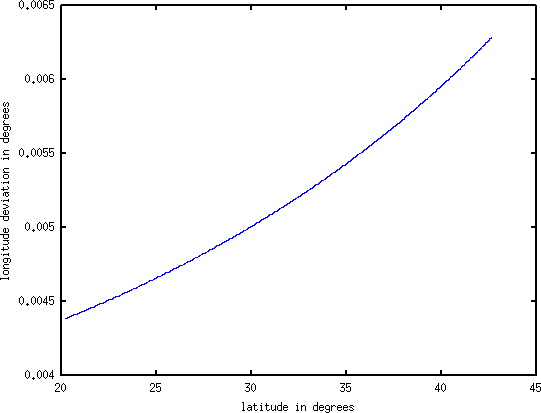
\includegraphics[width=0.48\textwidth]{fxy-degree.png}
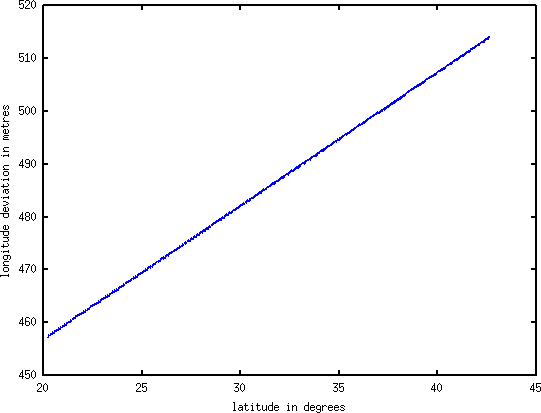
\includegraphics[width=0.48\textwidth]{fxy-metre.png}
\end{center}
\caption{$f_x(110.16,y)$. Left: longitude deviation (y-axis) is in degrees;
right: in metres.}
\label{fig:fxy-degree}
\end{figure}

Figure~\ref{fig:fxy-degree}(left) shows the plot, $f_x(110.16,y)$. The curve
looks like a second order curve, but if we go that direction, it's going to be
very tough.
It is a lot simpler if we measure the deviation in meters rather
than degrees.

\noindent
\verb|> plot(y,dx.*cos(y./180.*pi).*6371000.*pi./180)| \hfill
Figure~\ref{fig:fxy-degree}(right)

Figure~\ref{fig:fxy-degree}(right) shows the plot where the deviation is
measured in meters.
It's a linear function, thus we can do a simple linear regression.
\begin{verbatim}
> dx=dx.*cos(y./180.*pi).*6371000.*pi./180;
> mx=[ones(size(y)),y]; std(mx*(pinv(mx)*dx)-dx)
ans =  0.14664
> pinv(mx)*dx
ans =
   406.3954
     2.5241
\end{verbatim}
The standard error, 0.14664 meters, is acceptable.
The final function is
\begin{equation}
f_x(110.16,y)=406.3954+2.5241y
\end{equation}
After trying out other constant longitudes,
we find out that the two coefficients are different for different longitude.
We have
\begin{equation}
f_x(x,y)=g_1(x)+g_2(x)\times y
\end{equation}
where $g_1(x)$ and $g_2(x)$ are not yet known.

In the following analysis, we will measure $x$ and $y$ in degrees, while
measure $f_x(x,y)$ and $f_y(x,y)$ in meters. It makes our life a lot easier.

\subsection{$f_y(x, const)$}
$f_y(x, const)$ seems to be the second easiest one. It's quite obvious that
there are sinusoidal and linear components in the function. To find out the
frequency of the sinusoidal components, we do a Fourier transform.

\begin{verbatim}
> data=load("-ascii", "inx-f-39.txt");
> x=data(:,1);
> size(x)
ans =
   9116      1
> x(1)
ans =  73.655
> x(9116)
ans =  119.23
> dy=data(:,4).*(6371000*pi/180);
\end{verbatim}
\verb|> plot(x,dy)| \hfill Figure~\ref{fig:fyx-fft}(left) \\
\verb|> plot(abs(fft(dy)))| \hfill Figure~\ref{fig:fyx-fft}(right)

\begin{figure}[htb]
\begin{center}
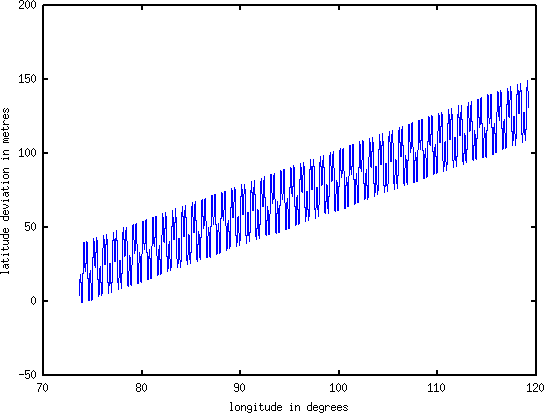
\includegraphics[width=0.48\textwidth]{fyx-data.png}
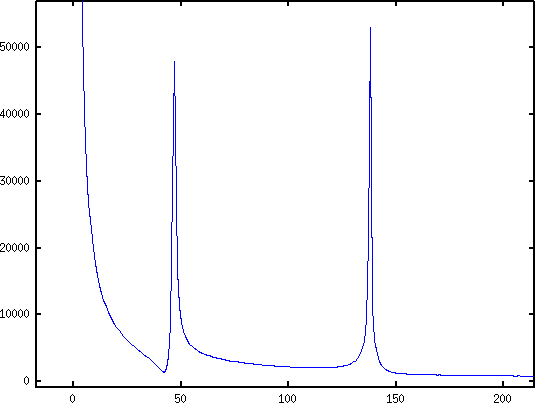
\includegraphics[width=0.48\textwidth]{fyx-fft.png}
\end{center}
\caption{$f_y(x,39.36)$. Left: the data points; right: FFT of the data}
\label{fig:fyx-fft}
\end{figure}

Figure~\ref{fig:fyx-fft}(left) shows the data and
Figure~\ref{fig:fyx-fft}(right) shows the data in frequency domain.
The two peaks in the frequency domains are at 47 and 138,
thus the frequencies are 46/45.575=1.0093 and 137/45.575=3.0060, where
45.575=119.23-73.655 is the range of x.
Since the range of x is not multiple of the periods, we don't get exact
results, but after cutting the range, the exact results are 1 and 3.
We then try to model it using $b+kx+a_1sin(2\pi x)+a_2cos(2\pi x)+a_3cos(6\pi
x)+a_4cos(6\pi x)$.

\begin{verbatim}
> mx=[ones(size(x)),x,sin(2.*pi.*x),cos(2.*pi.*x),sin(6.*pi.*x),\
  cos(6.*pi.*x)];
> std(mx*(pinv(mx)*dy)-dy)
ans =  0.38114
\end{verbatim}
\verb|> plot(x,dy,x,dy-mx*(pinv(mx)*dy))| \hfill Figure~\ref{fig:fyx-lc}

\begin{figure}[htb]
\begin{center}
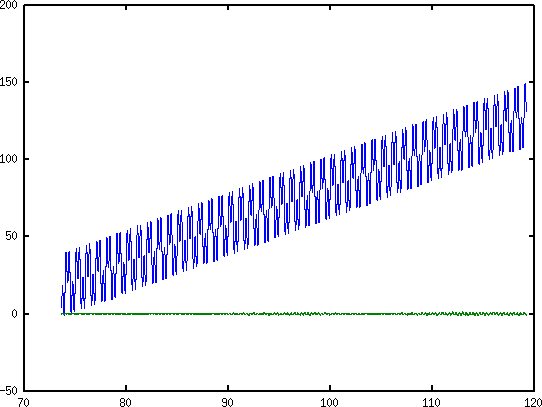
\includegraphics[width=0.48\textwidth]{fyx-lc.png}
\end{center}
\caption{The data (blue) and the regression error (green).}
\label{fig:fyx-lc}
\end{figure}
The standard error, 0.38114, is acceptable.
We can also see this in Figure~\ref{fig:fyx-lc}.
The regression error (difference between the data and our function) is close
to zero.
Let's see the coefficients:

\begin{verbatim}
> pinv(mx)*dy
ans =
  -160.45195
     2.42764
    13.33287
    -0.27150
    13.30099
    -0.82075
\end{verbatim}

We can combine sin and cos of the same frequency.

\begin{verbatim}
> atan(0.82075/13.30099)
ans =  0.061628
> atan(0.27150/13.33287)
ans =  0.020360
> mx=[ones(size(x)),x,sin(2.*pi.*x-0.020360),sin(6.*pi.*x-0.061628)];
> std(mx*(pinv(mx)*dy)-dy)
ans =  0.38114
> pinv(mx)*dy
ans =
  -160.4519
     2.4276
    13.3356
    13.3263
\end{verbatim}
So the function is
\begin{eqnarray}
f_y(x,39.36) & = & -160.45195+2.42764x+13.33287sin(2\pi x) \nonumber \\
             &   & -0.27150cos(2\pi x)+13.30099cos(6\pi x)-0.82075cos(6\pi x) \nonumber \\
             & = & -160.45195+2.42764x+13.3356sin(2\pi x-0.061628) \nonumber \\
             &   & +13.3263cos(6\pi x-0.020360)
\end{eqnarray}

After trying out other constant latitudes, we find out that the first two
coefficients to be changing but the last 4 coefficients to be fixed.
Thus, we know
\begin{eqnarray}
f_y(x,y) & = & g_1(y)+g_2(y)x+13.3356sin(2\pi x-0.061628) \nonumber \\
         &   & +13.3263cos(6\pi x-0.020360)
\end{eqnarray}
where $g_1(y)$ and $g_2(y)$ are not yet known.

\subsection{$f_x(x, const)$}
Similar to previous one, we use Fourier transform to find out the sinusoidal
components first.
\begin{verbatim}
> data=load("-ascii", "inx-f-39.txt");
> x=data(:,1);
> dx=data(:,3).*cos(39.36./180.*pi).*6371000.*pi./180;
\end{verbatim}
\verb|> plot(x,dx)| \hfill Figure~\ref{fig:fxx-fft}(left) \\
\verb|> plot(abs(fft(dx)))| \hfill Figure~\ref{fig:fxx-fft}(right) \\

\begin{figure}[htb]
\begin{center}
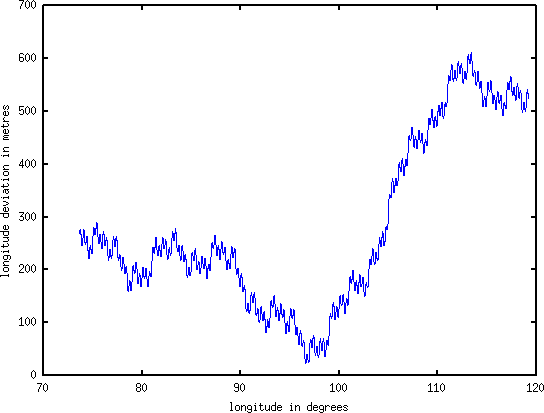
\includegraphics[width=0.48\textwidth]{fxx-data.png}
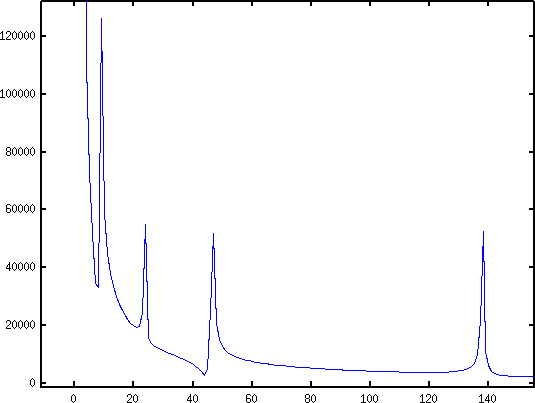
\includegraphics[width=0.48\textwidth]{fxx-fft.png}
\end{center}
\caption{$f_x(x,39.36)$. Left: the data points; right: FFT of the data}
\label{fig:fxx-fft}
\end{figure}

Figure~\ref{fig:fxx-fft}(left) shows the curve that we are going to fit.
Figure~\ref{fig:fxx-fft}(right) shows the frequency domain.
The peaks are at 9, 24, 47 and 138, so the frequencies are 8/45.575=0.17553,
23/45.575=0.50466, 46/45.575=1.0093 and 137/45.575=3.0060.
The exact frequencies are 1/6, 1/2, 1 and 3.
Now, we try to fit the curve with the 4 sinusoidal components and
a linear component.
\begin{verbatim}
> mx=[ones(size(x)),x,sin(pi.*x./3),cos(pi.*x./3),sin(pi.*x),\
  cos((pi.*x)),sin(2.*pi.*x),cos(2.*pi.*x),sin(6.*pi.*x),\
  cos((6.*pi.*x))]; std(mx*(pinv(mx)*dx)-dx)
ans =  119.96
> plot(x,dx,x,dx-mx*(pinv(mx)*dx))
\end{verbatim}
\begin{figure}[htb]
\begin{center}
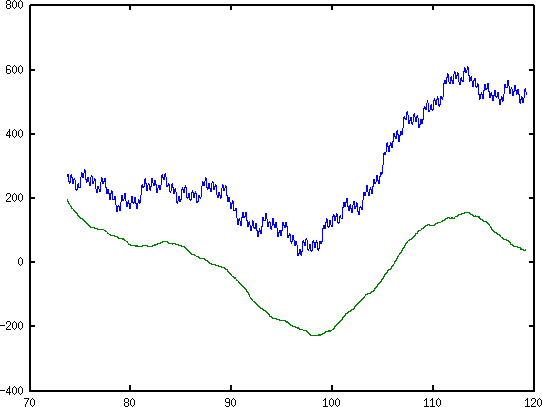
\includegraphics[width=0.48\textwidth]{fxx-lc1.png}
\end{center}
\caption{The data (blue) and the regression error (green).}
\label{fig:fxx-lc1}
\end{figure}
The standard error 119.96 meters is not acceptable.
To see it, we plot the difference in Figure~\ref{fig:fxx-lc1}.
It seems that there are some low frequency components.
We can deal with low frequency components with a bunch of polynomials.
\begin{verbatim}
> mx=[ones(size(x)),(x./mean(x)),(x./mean(x)).^2,(x./mean(x)).^3,\
  (x./mean(x)).^4,(x./mean(x)).^5,(x./mean(x)).^6,(x./mean(x)).^7,\
  (x./mean(x)).^8,(x./mean(x)).^9,sin(pi.*x./3),cos(pi.*x./3),\
  sin(pi.*x),cos((pi.*x)),sin(2.*pi.*x),cos(2.*pi.*x),sin(6.*pi.*x),\
  cos((6.*pi.*x))]; std(mx*(pinv(mx)*dx)-dx)
ans =  0.78555
\end{verbatim}
It fits well with a 9-order polynomial.
Note that we divide $x$ by $mean(x)$ to make sure the values in the matrix
have low dynamic range so as to reduce numeric error.
Mathematically, they don't make a difference.
To see how our polynomial works, we can plot the polynomial and compare with
the data (see Figure~\ref{fig:fxx-lc2}).
\begin{verbatim}
> coeff=pinv(mx)*dx;
> coeff(11:18)=0
coeff =
   1.3529e+08
  -1.3862e+09
   6.2344e+09
  -1.6167e+10
   2.6655e+10
  -2.8993e+10
   2.0816e+10
  -9.5166e+09
   2.5150e+09
  -2.9286e+08
   0.0000e+00
   0.0000e+00
   0.0000e+00
   0.0000e+00
   0.0000e+00
   0.0000e+00
   0.0000e+00
   0.0000e+00
> plot(x,dx,x,mx*coeff)
\end{verbatim}

\begin{figure}[htb]
\begin{center}
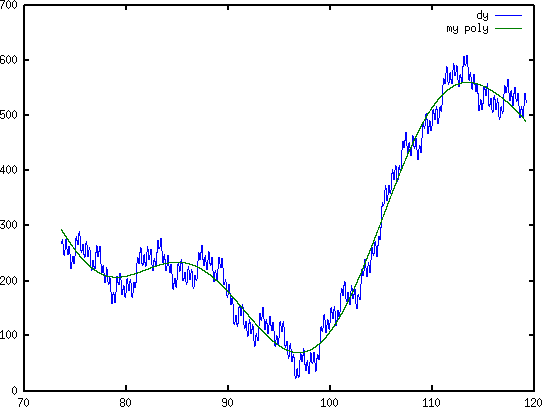
\includegraphics[width=0.6\textwidth]{fxx-lc2.png}
\end{center}
\caption{9-order polynomial (green) and 9-order polynomial + sinusoidal (blue)}
\label{fig:fxx-lc2}
\end{figure}

Although the 9-order polynomial fits the data well (error is 0.79 meters),
the function is ugly.
After lots of tries\footnote{
Most of the time has been spent here, but there is nothing to say about it
because it's simply trying different functions.
There are still a little bit of technique though.
For example, the two green peaks in Figure~\ref{fig:fxx-lc2} have distance
about 24 in x-axis, thus there might be a sinusoidal component of period 24.
}, I figured out that the low frequency
component actually consists of a quadratic curve and two sinusoidal wave of
period 60 and 24.
Using this model, the regression error is 0.39 meters and the function is
simple and beautiful.
\begin{verbatim}
> mx=[ones(size(x)),x,x.*x,sin(pi.*x./30),cos(pi.*x./30),\
  sin(pi.*x./12),cos(pi.*x./12),sin(pi.*x./3),cos(pi.*x./3),\
  sin(pi.*x),cos((pi.*x)),sin(2.*pi.*x),cos(2.*pi.*x),sin(6.*pi.*x),\
  cos((6.*pi.*x))]; std(mx*(pinv(mx)*dx)-dx)
ans =  0.38668
> pinv(mx)*dx
ans =
   1.2052e+03
  -1.8404e+01
   9.4022e-02
   8.3824e-01
   2.0044e+02
  -7.0435e+01
  -7.0449e+01
  -2.6699e+01
   9.1218e-02
  -1.3342e+01
   1.3044e-01
   1.3342e+01
  -2.7504e-01
   1.3306e+01
  -8.2298e-01
\end{verbatim}

Now let's merge sin and cos.
\begin{verbatim}
> atan(2.0044e+02/8.3824e-01)
ans =  1.5666
> atan(7.0449e+01/7.0435e+01)
ans =  0.78550
> atan(9.1218e-02/2.6699e+01)
ans =  0.0034165
> atan(1.3044e-01/1.3342e+01)
ans =  0.0097763
> atan(2.7504e-01/1.3342e+01)
ans =  0.020612
> atan(8.2298e-01/1.3306e+01)
ans =  0.061772
> mx=[ones(size(x)),x,x.*x,sin(pi.*x./30+1.5666),sin(pi.*x./12+0.78550),\
  sin(pi.*x./3-0.0034165),sin(pi.*x-0.0097763),sin(2.*pi.*x-0.020612),\
  sin(6.*pi.*x-0.061772)]; std(mx*(pinv(mx)*dx)-dx)
ans =  0.38668
> pinv(mx)*dx
ans =
   1.2051e+03
  -1.8402e+01
   9.4012e-02
   2.0045e+02
  -9.9620e+01
  -2.6699e+01
  -1.3343e+01
   1.3344e+01
   1.3332e+01
\end{verbatim}

Finally, we have
\begin{eqnarray}
f_x(x,39.36) & = & 1205.1 -18.402x +0.094012x^2 +200.45sin(\pi x/30+1.5666) \nonumber \\
             &   & -99.62sin(\pi x/12+0.78550) -26.699sin(\pi x/3-0.0034165) \nonumber \\
             &   & -13.343sin(\pi x-0.0097763) +13.344sin(2\pi x-0.020612) \nonumber \\
             &   & +13.332sin(6\pi x-0.061772)
\end{eqnarray}
To see how the components fit the data, we can graduately add
the higher frequency components. Figure 5.5 shows this this idea. Figure 5.6 is
a zoomed in region in Figure 5.5. The first function (in red) is the quadratic
function $1205.1 -18.402x +0.094012x^2$. The second function (in green) adds
one sinusoidal component to it: $1205.1 -18.402x +0.094012x^2 +200.45sin(\pi
x/30+1.5666)$. The third function (in blue) adds one more sinusoidal component
to it, etc.
\begin{figure}[htb]
\begin{center}
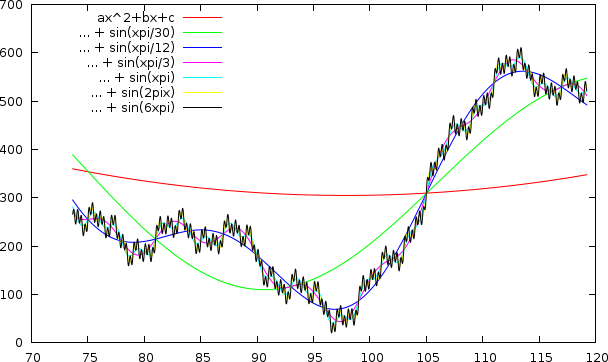
\includegraphics[width=0.48\textwidth]{fxx-lc3.png}
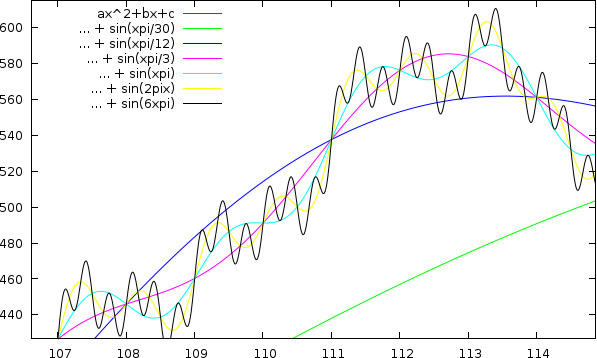
\includegraphics[width=0.48\textwidth]{fxx-lc4.png}
\end{center}
\caption{Decomposition of Components.
Left: overall; right: zoomed in.
The first function (red) has only the lowest frequency component.
The second function (green) adds the second lowest frequency component to the
first function.
The third (blue) adds another component, etc.}
\label{fig:fxx-lc3}
\end{figure}

After trying out other constant latitude, we found that only the first two
coefficients are affected by latitude. The rest of the coefficients do not
change. Thus, we have
\begin{eqnarray}
f_x(x,y) &=& g_1(y) -g_2(y)x +0.094012x^2 +200.45sin(\pi x/30+1.5666) \nonumber \\
         & & -99.62sin(\pi x/12+0.78550) -26.699sin(\pi x/3-0.0034165) \nonumber \\
         & & -13.343sin(\pi x-0.0097763) +13.344sin(2\pi x-0.020612) \nonumber \\
         & & +13.332sin(6\pi x-0.061772)
\end{eqnarray}
where $g_1(y)$ and $g_2(y)$ are not yet known.

\subsection{$f_y(const, y)$}

The process of finding $f_y(const, y)$ is similar to $f_x(x, const)$, except
that the two high frequency sinusoidal components do not appear in $f_y(const,
y)$.
\begin{verbatim}
> data=load("-ascii", "iny-a-110.txt");
> y=data(:,2);
> dy=data(:,4).*(6371000*pi/180);
> my=[ones(size(y)),y,y.*y,sin(pi.*y./30),cos(pi.*y./30),\
  sin(pi.*y./12),cos(pi.*y./12),sin(pi.*y./3),cos(pi.*y./3),\
  sin(pi.*y),cos((pi.*y))]; std(my*(pinv(my)*dy)-dy)
ans =    0.16683
> pinv(my)*dy
ans =
       162.1
     -22.422
     0.41569
     -172.78
      56.189
     -104.96
     -29.351
      13.251
      23.113
     -13.357
   -0.061311
> atan(56.189/-172.78)
ans =   -0.31442
> atan(-29.351/-104.96)
ans =    0.27267
> atan(23.113/13.251)
ans =     1.0502
> atan(-0.061311/-13.357)
ans =  0.0045901
> my=[ones(size(y)),y,y.*y,sin(pi.*y./30-0.31442),\
  sin(pi.*y./12+0.27267),sin(pi.*y./3+1.0502),\
  sin(pi.*y+0.0045901)]; std(my*(pinv(my)*dy)-dy)
ans =    0.16683
> pinv(my)*dy
ans =
      162.09
     -22.422
     0.41568
     -181.69
     -108.99
      26.643
     -13.357
\end{verbatim}

We have
\begin{eqnarray}
f_y(110.16,y) &=& 162.09-22.422y+0.41568y^2 \nonumber \\
              & & -181.69sin(\pi y/30-0.31442)-108.99sin(\pi y/12+0.27267) \nonumber \\
              & & +26.643sin(\pi y/3+1.05)-13.357sin(\pi y-0.00459) \\
f_y(x,y)      &=& g_1(x)+g_2(x)y+0.41568y^2 \nonumber \\
              & & -181.69sin(\pi y/30-0.31442)-108.99sin(\pi y/12+0.27267) \nonumber \\
              & & +26.643sin(\pi y/3+1.05)-13.357sin(\pi y-0.00459)
\end{eqnarray}

\section{The final 2D case: $f_x(x,y)$ and $f_y(x,y)$}
With out too much effort, we have found out the two functions:

\begin{eqnarray}
f_x(x,y) &=& 1598.1-23.605x -8.4345y +0.09933xy +0.10069x^2 \nonumber \\
          & & +199.1cos(\pi(x+0.017)/30) -99.772sin(\pi(x+0.0039)/12+\pi/4) \nonumber \\
          & & -26.687sin(\pi(x-0.0039)/3) -13.345sin(\pi(x-0.0039)) \nonumber \\
          & & +13.338sin(2\pi(x-0.0039)) +13.331sin(6\pi(x-0.0039)) \\
f_y(x,y) &=& -36.759 +1.5218x +10.002y -0.10032xy -0.03661y^2 \nonumber \\
         & & -217.44cos(\pi(y+8.143)/30)+106.41sin(\pi(y+1.1)/12) \nonumber \\
         & & -26.697sin(\pi(y+1)/3) +13.335sin(\pi y) \nonumber \\
         & & -13.329sin(2\pi(x-0.0039)) -13.319sin(6\pi(x-0.0039))
\end{eqnarray}
The standard errors are 0.43747 and 0.44031 meters respectively.

To verify the correctness, we can 

\end{document}
